%!TEX root = SISC_elastic_3d.tex
\subsection{Energy conservation test}\label{conserved_energy}
To verify the energy conservation property of the scheme, we perform computation without external source term, but with a Gaussian initial profile centered at the origin of the computational domain. The computational domain is chosen to be the same as in Sec.~\ref{convergence_study}. The material is discontinuous: for the fine domain $\Omega^f$,  the density varies according to
\[\rho^f(x^{(1)},x^{(2)},x^{(3)}) = 3 + \sin(2x^{(1)}+0.3)\cos(x^{(2)}+0.3)\sin(2x^{(3)}-0.2),\] 
and material parameters satisfy
\[\mu^f(x^{(1)},x^{(2)},x^{(3)}) = 2 + \cos(3x^{(1)}+0.1)\sin(3x^{(2)}+0.1)\sin(x^{(3)})^2,\]
\[\lambda^f(x^{(1)},x^{(2)},x^{(3)}) = 15 + \cos(x^{(1)}+0.1)\sin(4x^{(2)}+0.1)\sin(3x^{(3)})^2;\]
for the coarse domain $\Omega^c$, the density varies according to
\[\rho^c(x^{(1)},x^{(2)},x^{(3)}) = 2 + \sin(x^{(1)}+0.3)\sin(x^{(2)}+0.3)\sin(2x^{(3)}-0.2),\] 
and material parameters satisfy
\[\mu^c(x^{(1)},x^{(2)},x^{(3)}) = 3 + \sin(3x^{(1)}+0.1)\sin(3x^{(2)}+0.1)\sin(x^{(3)}),\]
\[\lambda^c(x^{(1)},x^{(2)},x^{(3)}) = 21 + \cos(x^{(1)}+0.1)\cos(x^{(2)}+0.1)\sin(3x^{(3)})^2.\]
The initial Gaussian profile is given by ${\bf C}(\cdot,0) = {\bf F}(\cdot,0) = {\bf u}(\cdot,0) = (u_1(\cdot,0),u_2(\cdot,0),u_3(\cdot,0))^T$ with
\begin{align*}
	u_1(\cdot,0) &= \mbox{exp}\left(-\frac{(x^{(1)}-\pi)^2}{0.1}\right)\mbox{exp}\left(-\frac{(x^{(2)}-\pi)^2}{0.1}\right)\mbox{exp}\left(-\frac{(x^{(3)}-\pi)^2}{0.1}\right),\\
	u_2(\cdot,0) &= \mbox{exp}\left(-\frac{(x^{(1)}-\pi)^2}{0.2}\right)\mbox{exp}\left(-\frac{(x^{(2)}-\pi)^2}{0.2}\right)\mbox{exp}\left(-\frac{(x^{(3)}-\pi)^2}{0.2}\right),\\
	u_3(\cdot,0) &= \mbox{exp}\left(-\frac{(x^{(1)}-\pi)^2}{0.1}\right)\mbox{exp}\left(-\frac{(x^{(2)}-\pi)^2}{0.2}\right)\mbox{exp}\left(-\frac{(x^{(3)}-\pi)^2}{0.2}\right).
\end{align*}
 The grid spacing in the parameter space for the coarse domain $\Omega^c$ is $2h_1 = 2h_2 = 2h_3 = \frac{\pi}{24}$ and for the fine domain $\Omega^f$ is $h_1 = h_2 = h_3 = \frac{\pi}{48}$, that is we have $25\times25\times13$ grid points in the coarse domain $\Omega^c$ and $49\times49\times25$ grid points in the fine domain $\Omega^f$. 

For the semi-discrete approximation, the energy is given by $({\bf f}_t,({\rho}^h\otimes{\bf I}){\bf f}_t)_h + \mathcal{S}_h({\bf f},{\bf f}) + ({\bf c}_t,({\rho}^{2h}\otimes{\bf I}){\bf c}_t)_{2h} + \mathcal{S}_{2h}({\bf c},{\bf c})$, see (\ref{semi_energy_1}). By using the same approach as for the isotropic elastic wave equation, see \cite{petersson2015wave,sjogreen2012fourth},  the expression for the full discrete energy reads as
\begin{align*}
&E^{n+1/2} = \left|\left|(\rho^h\otimes {\bf I})^{\frac{1}{2}}\frac{{\bf f}^{n+1}-{\bf f}^n}{\Delta t}\right|\right|_h^2 + S_h({\bf f}^{n+1},{\bf f}^n) - \frac{(\Delta t)^2}{12}\Big((J^h\otimes{\bf I})^{-1}\mathcal{L}^h{\bf f}^{n+1},(J^h\otimes{\bf I})^{-1}\mathcal{L}^h{\bf f}^n\Big)_h\\
&+ \left|\left|(\rho^{2h}\otimes{\bf I})^{\frac{1}{2}}\frac{{\bf c}^{n+1}-{\bf c}^n}{\Delta t}\right|\right|_{2h}^2 + S_{2h}({\bf c}^{n+1},{\bf c}^n) - \frac{(\Delta t)^2}{12}\Big((J^{2h}\otimes{\bf I})^{-1}\wt{\mathcal{L}}^{2h}{\bf c}^{n+1},(J^{2h}\otimes{\bf I})^{-1}\wt{\mathcal{L}}^{2h}{\bf c}^n\Big)_{2h}.
\end{align*}
We present the relative change in full discrete energy, $(E^{n+1/2}-E^{1/2})/E^{1/2}$, as a function of time with $t\in[0,120]$ in Figure \ref{discrete_energy}. This corresponds to $6186$ time steps. Our numerical results show that the full discrete energy remains constant up to round-off error.
\begin{figure}[htbp]
	\centering
	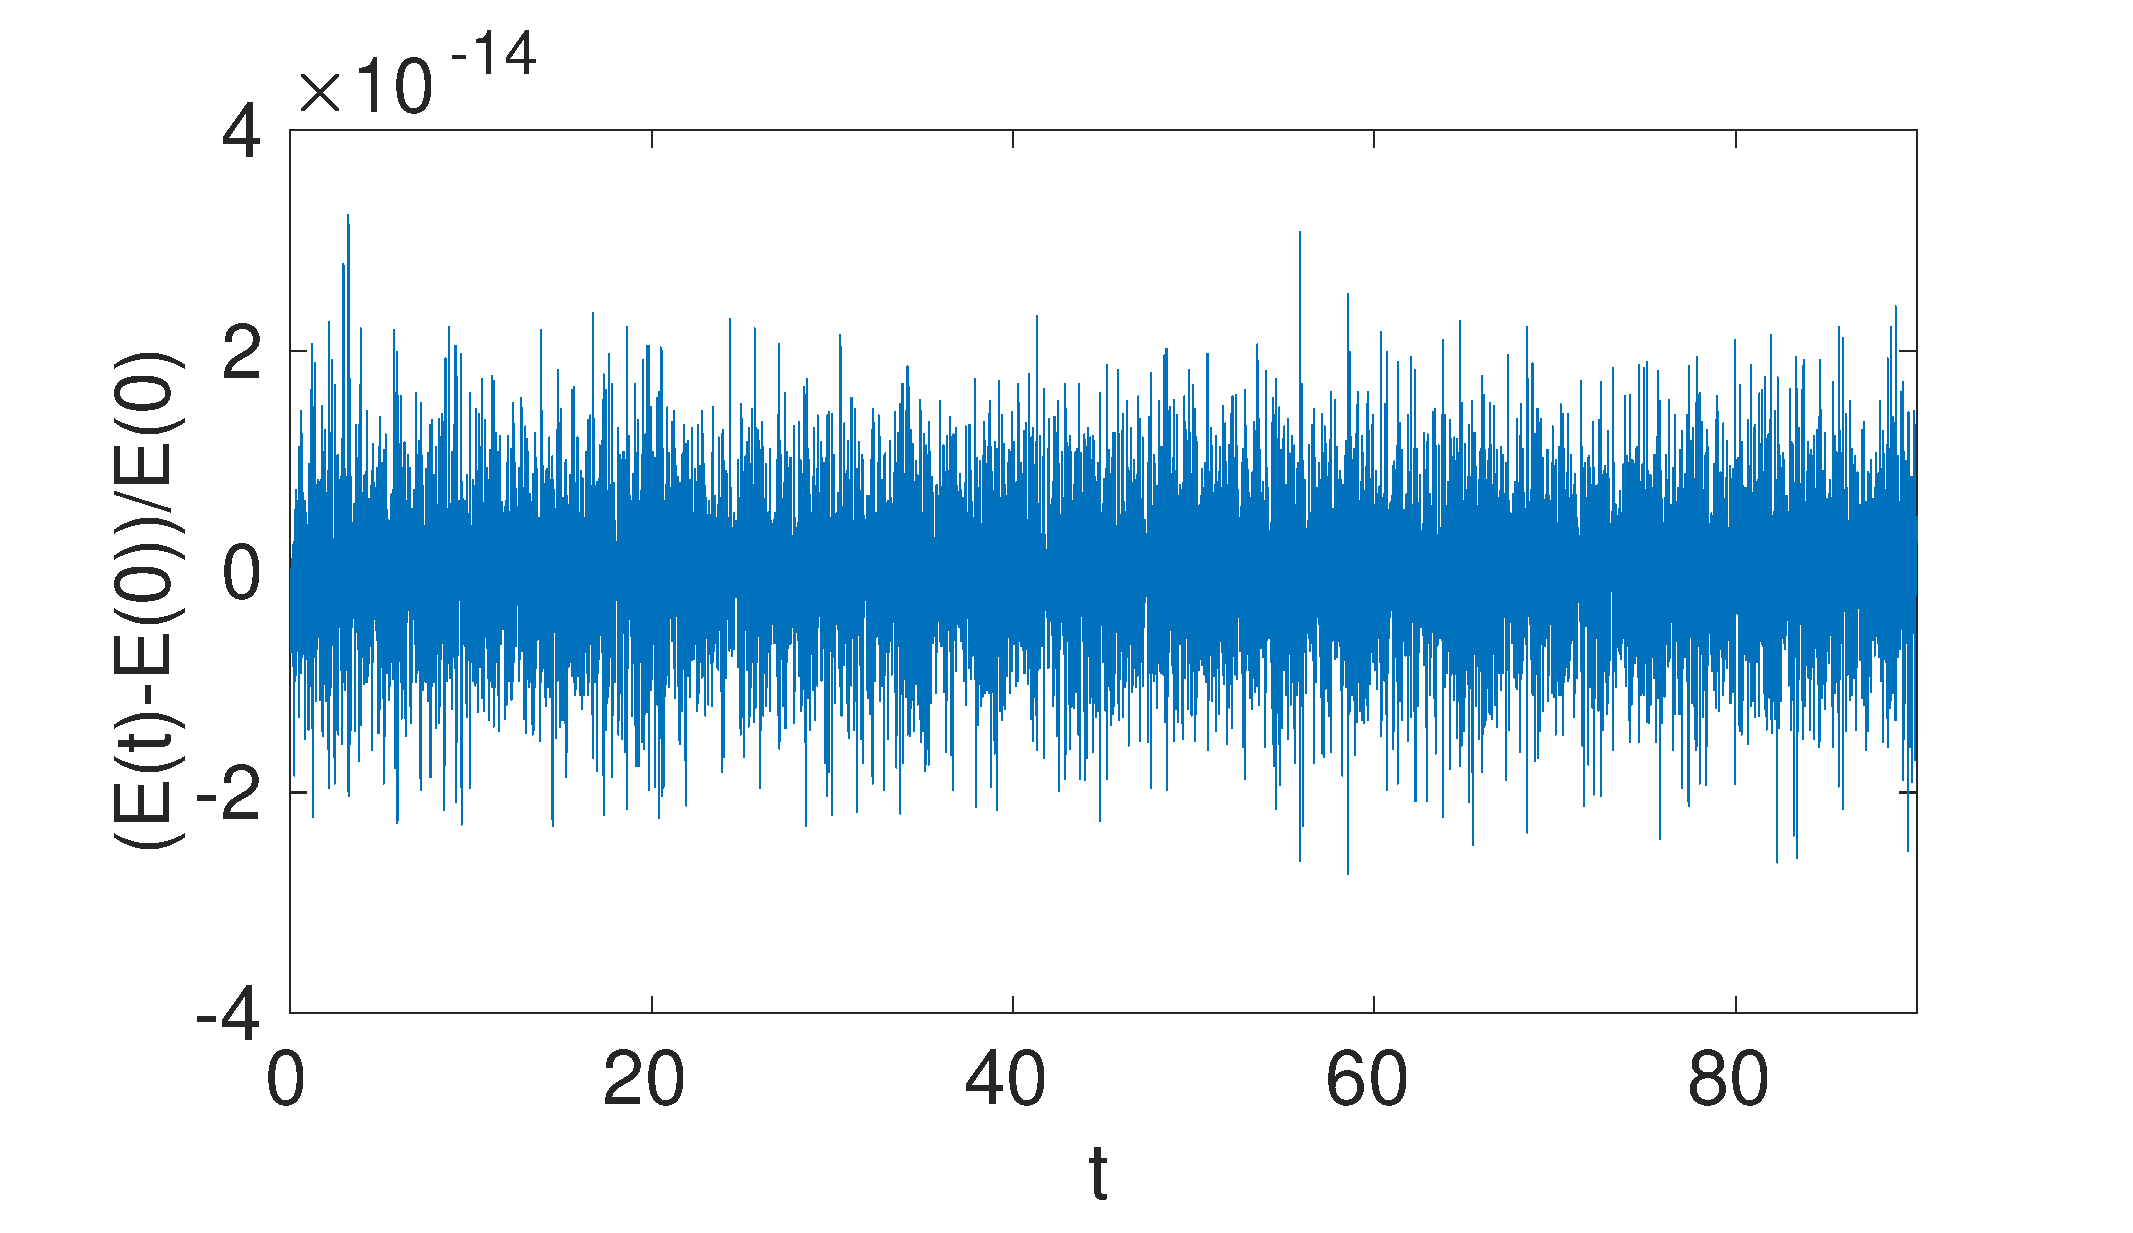
\includegraphics[width=0.6\textwidth,trim={0cm 0cm 0cm 0cm}, clip]{discrete_energy.eps}
	\caption{The relative change in fully discrete energy as a function of time. Here, $t = 120$ corresponds to $6186$ time steps.}\label{discrete_energy}
\end{figure}


